
%% ==================================================================================================
%%
\documentclass[12pt]{book}
\usepackage{amsfonts}
\usepackage{amsmath}
\usepackage{amssymb}
\usepackage{graphicx}
\usepackage{hyperref}
\usepackage{float}
\usepackage{verbatim}
\usepackage{xlop} %% for multiplication https://tex.stackexchange.com/questions/11702/how-to-present-a-vertical-multiplication-addition
\usepackage{listings} %% to format generic computer code
\usepackage{lmodern} % for bold teletype font
\usepackage{minted} % colour Java code

\usepackage{tasks}
%\NewTasks[style=enumerate,counter-format=tsk[A].,label-width=3ex]{choice}[\item](4)

%% =======   set page margins    =======
\setlength{\textheight}{10in}
\setlength{\textwidth}{7.4in}
\setlength{\topmargin}{-0.75in}
\setlength{\oddsidemargin}{-0.5in}
\setlength{\evensidemargin}{-0.5in}
\setlength{\parskip}{0.15in}
\setlength{\parindent}{0in}

%%  for European long division
% https://tex.stackexchange.com/questions/432435/how-to-set-up-european-french-style-long-division-in-tex
\newcommand\frdiv[5]{%
    \[
    \renewcommand\arraystretch{1.5}
    \begin{array}{l| l}
    #1 & #2 \\
    \cline{2-2}
    #3 & #4 \\
    \cline{1-1}
    #5 & \\
    \end{array}
    \]
}

%%  for European long division


%% ==================================================================================================

\begin{document}

\newcommand{\reporttitle}{Assignment 3}
\newcommand{\reportauthorOne}{Kien Do}
\newcommand{\cidOne}{300163370}
\input{titlePage/titlepage.txt}



%% ==================================================================================================

%%%%%%%%%%%% PROBLEMS START HERE

\begin{enumerate}
    %% ============================   New Item   ============================
    \item \textbf{Answer}\\
    
    Below is the recursion definition that is filled in,
    
    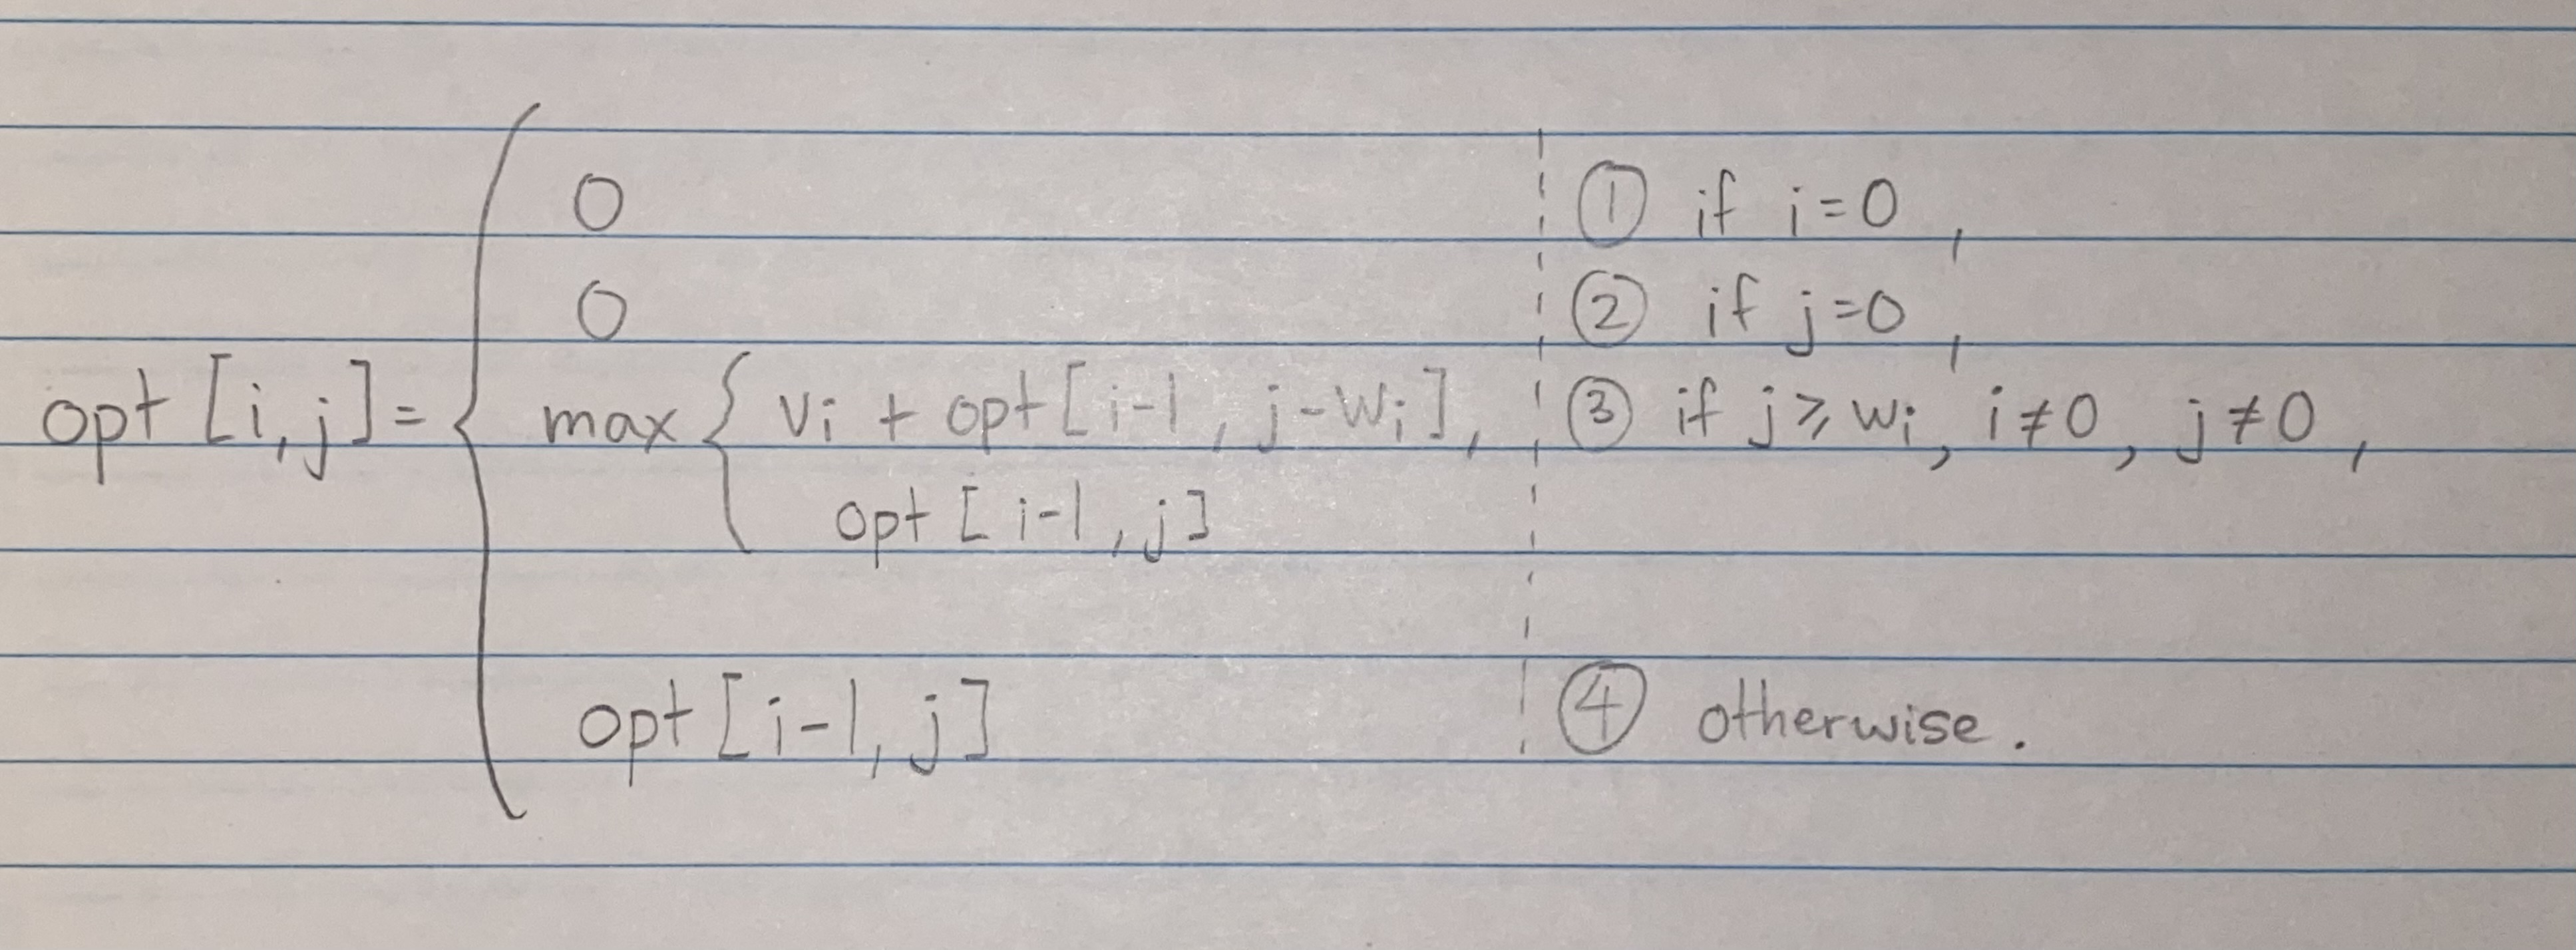
\includegraphics[scale=0.125]{q1.png}\\
    
    Below is the justification (for my own reference).\\
    
    1. No object, therefore the optimal value is 0.\\
    2. Max weight is 0, and since $w_i > 0$, no such $w_i$ can satisfy the condition.\\
    3. The optimal value is the maximum of the following two cases:\\
    --- The value of the current item $v_i$ \textunderscore{plus} the existing optimal value for the remaining weight after including item $i$, and\\
    --- the existing optimal value from the previous calculation.\\
    4. The optimal value is simply the existing optimal value from the previous calculation.\\
    
    \newpage
    
    %% ============================   New Item   ============================
    \item \textbf{Answer}
    
    Following the recursive algorithm proposed in question 1, we can solve the knapsack problem with the given values using the matrix method of dynamic programming.\\
    
    We are given,
    $$W = 11, \,n = 6$$
    as well as the weight of each item,
    $$w_1 = 2, w_2 = 3, w_3 = 2, w_4 = 9, w_5 = 3, w_6 = 2$$
    and the value of each item,
    $$v_1 = 7, v_2 = 1, v_3 = 6, v_4 = 18, v_5 = 22, v_6 = 28$$
    
    The following matrix can be produced.
    
    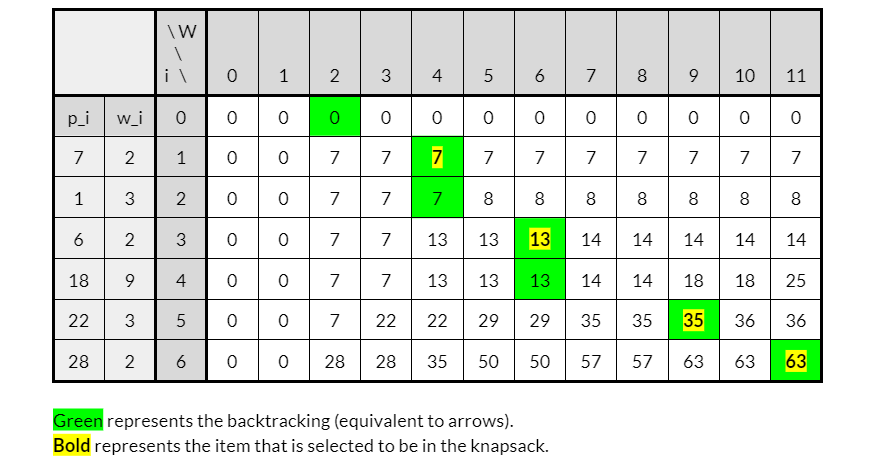
\includegraphics[scale=0.9]{q2.png}\\
    
    \textbf{Result:}
    
    --- The items included in the knapsack are items 6, 5, 3, and 1.\\
    --- The total weight is 2 + 3 + 2 + 2 = 9, which is less than the maximum weight, W = 11.\\
    --- The total value is 63.

    
\end{enumerate}

\end{document} 
